\subsection{Mass distribution from lensing} \label{sec:results_lensing}

\paragraph{Image positions.} We determine the positions of the lensing images by first subtracting a smooth model for the galaxy's surface brightness from the original image. As models we use MGE fits and IRAF ellipse fits  (see Sections \ref{sec:MGE_theo} and \ref{sec:MGE_results})  to the galaxy in each the F450W and F814W filter. (For example the MGE we use for F814W is the MGE given in Table \ref{tab:MGEF814W} convolved with the PSF in Table \ref{tab:PSFMGEF814W}.) The lensing images become then visible in the residuals (see Figure \ref{fig:lens_just_imgpos}), in which we smooth out noise smaller than the PSF. Because the lensing images are extended, we use the position of the brightest pixel in each of the images. We also use the F450W-MGE subtracted residuals from \citet{SWELLSIII}. The lensing positions as determined from the latter are given in Table \ref{tab:lenspos}. The scatter of lensing positions as determined from subtracting different surface brightness models from the galaxy in different filters gives an error of $\pm 1$ pixel on the image positions. We find slightly different positions for the peak of the surface brightness in the different filters and apply correspondingly an error of one diagonal pixel to the brightness peak in the F450W image which we use as center of the galaxy.
\\Eight image position coordinates allow us to fit a lens mass model with only $<8$ free parameters. We therefore do not fit Fourier components $(a_k,b_k)$ with $k > 3$.
\\Even though the constraints from the image positions on $\alpha$ is very weak, we were however able to show that the image positions in Table \ref{tab:lenspos} are consistent with a model with flat rotation curve. In the following we therefore set $\alpha=1$.

\begin{table}
\centering
\begin{minipage}{70mm}
\begin{tabular}{r|rrrr|c}
\hline
  & A & B & C & D & G\\\hline
$x_i$ [pixel] & 12.1 & -8.5 & 21.7 & -3.3 & 0.5 $\pm \sqrt{2}$ \\
$y_i$ [pixel] & 16.6 & -10.4 & -0.5 & 19.2 & 0.5 $\pm \sqrt{2}$ \\
\hline
\end{tabular}
\caption{Positions of the lensing images (A-D) and the galaxy center (G) in Figure \ref{fig:lens_just_imgpos}. The image positions were determined from the lens subtracted image for J1331 in Figure 4 of \citet{SWELLSIII}, rotated to the $(x,y)$ coordinate system in Figure \ref{fig:lens_just_imgpos}. The pixel scale is 1 pixel = 0.05 arcsec and the error of each image position is $\pm$ 1 pixel.}
\label{tab:lenspos}
\end{minipage}
\end{table}


\paragraph{Best fit lens model.} The best fit lens model for the image positions in Table \ref{tab:lenspos} is given in the first column of Table \ref{tab:bestfitlensmodel}. Figure \ref{fig:lensbestfiteinsteincurves} shows the corresponding critical curve, caustic and Einstein radius, and the best fit source position. In this case, where $\alpha=1$, the critical curve is also an equidensity contour of the galaxy model \citep{EvansWitt}, which appears to have an elliptical mass distribution. This cricital curve is called \emph{tangential}, because of the tangential orientation of the images close to it. The source is located close to a cusp of the diamond-shaped caustic: a lensing configuration for which we indeed expect four images. This is a good indication that indeed all four images are indeed lensing images of the same object. Figure \ref{fig:lensbestfittimedelay} overplots the smoothed residuals from the F450W image subtracted by the IRAF ellipse fit to the surface brightness with the contours of the best fit model's time delay surface. This demonstrates that, although we did not include any information about the shape of the lensing images in the fit, it is consistent with the predicted distortion for an extended source by the best fit lens model.
\\To estimate how the uncertainties in the determination of the image positions and galaxy center affect the results, we Monte Carlo sample random positions from a two-dimensional Normal distribution centered at the positions in Table \ref{tab:lenspos} and a standard deviation corresponding to the measurement error. A Gaussian fit to the resulting distributions of best fit values leads to the constraints on the shape parameters and Einstein quantities in the second column in Table \ref{tab:bestfitlensmodel}. We therefore constrain the Einstein radius to within 2\%, $R_\text{ein} = (0.91 \pm 0.02)$ arcsec and the projected mass within the critical curve with a relative error of 4\%, $M_\text{crit} =(7.9\pm0.3)\cdot 10^{10} M_\odot$. Our measurement of $R_\text{ein}$ is consistent with that from \citet{SWELLSIII}, $R_\text{ein,SWELLS} = (0.96 \pm 0.04)$ arcsec (which used a singular isothermal ellipsoid as lens mass model and the intermediate-axis convention of the critical curve as the Einstein radius). The relative difference between our critical mass and that of \citet{SWELLSIII}, $M_\text{crit,SWELLS} =(8.86\pm0.61)\cdot 10^{10} M_\odot$, is 13\%.

%========================================================================================

\begin{table*}
\centering
\caption{Best fit lens model found from the peak image positions in Table \ref{tab:lenspos} (first column) following the procedure described in Section \ref{sec:lensing_theo} and assuming a flat rotation curve ($\alpha = 1$). The second column gives the corresponding best fit mean and standard deviation derived from Monte Carlo sampling of the Gaussian uncertainties around the image positions (column 2).}
\begin{tabular}{llrrclr}
\hline
 &  & \multicolumn{1}{c}{lens model for} &\multicolumn{4}{c}{lens model from Monte Carlo sampling  } \\
 &  & \multicolumn{1}{c}{peak image positions}  & \multicolumn{4}{c}{of image positions }  \\ \hline
Einstein radius      & $R_\text{ein}$ [arcsec]             & $0.907$ & $0.91$  & $\pm$ & $     0.02$ & ($2\%$)\\
Einstein mass        & $M_\text{ein}$ [$10^{10} M_\odot$]  & $7.72$  & $7.8 $  & $\pm$ & $      0.3$ & ($4\%$) \\
Critical mass        & $M_\text{crit}$ [$10^{10} M_\odot$] & $7.87$  & $7.9$   & $\pm$ & $      0.3$ & ($4\%$)\\
Source position      & $\xi$ [arcsec]                      & $0.095$ & $0.09 $ & $\pm$ & $     0.03$ & ($28\%$)\\
                     & $\eta$ [arcsec]                     & $0.107$ & $0.10 $ & $\pm$ & $     0.03$ & ($27\%$)\\
Fourier coefficients & $a_0$                               & $1.814$ & $1.82 $ & $\pm$ & $   0.04$ & (2\%)\\
                     & $a_2$                               & $0.012$ & $ 0.011 $ & $\pm$ & $    0.004$ & (35\%)\\
                     & $b_2$                               & $-0.057$ & $-0.06 $  & $\pm$ & $  0.01$ & (25\%)\\
                     & $a_3$                               & $-0.0001$& $0.0000 $ & $\pm$ & $   0.0006$ & \\
                     & $b_3$                               & $-0.0002$&$0.000 $   & $\pm$ & $  0.001$ & \\\hline
\end{tabular}  
\label{tab:bestfitlensmodel} 
\end{table*}

%========================================================================================

\begin{figure*}
\centering
\begin{subfigure}{.5\textwidth}
  \centering
  \includegraphics[width=.9\linewidth]{fig/lens_einstein.ps}
  \caption{Best fit critical curve, Einstein radius, caustic, source position.}
  \label{fig:lensbestfiteinsteincurves}
\end{subfigure}%
\begin{subfigure}{.5\textwidth}
  \centering
  \includegraphics[width=.9\linewidth]{fig/lens_timedelay.ps}
  \caption{Time delay surface.}
  \label{fig:lensbestfittimedelay}
\end{subfigure}
\caption{Best fit lens model in Table \ref{tab:bestfitlensmodel} found from the image positions. In the background we show the central region of J1331 in the F450W filter, subtracted by an Iraf Ellipse model of the F450W surface brightness and smoothed by boxcar smoothing of the order of the PSF size. The four bluish lensing images are clearly visible and we mark the brightness peaks in Table \ref{tab:lenspos} as well as the galaxy center (G) as red dots. The Einstein radius of the best fit lens model is shown as a red dotted circle. \emph{Panel (a)} Besides the image positions and Einstein radius, the critical curve (red solid line) is shown in the lens plane. The caustic (green solid line) corresponding to the critical curve and best fit source position (green dot), which are both located in the source plane, are shown as well. For $\alpha=1$ (which we assumed for our lens model) the critical curve is a contour of constant surface density of the mass model. \emph{Panel (b)} The yellow lines show (arbitrary) contours of the time delay surface given by Equation \ref{eq:timedelay} of the best fit lens model. Not only the position of the extrema, but also their shape is consistent with the observed, extended images, even though we did not use information about the image shape in the analysis. The other two right blobs (north east of A, south east of B) might be star forming regions of the background galaxy as well. [TO DO: Add A, B, C, D in the figure to make clear which image is which.]}
\label{fig:???}
\end{figure*}

%========================================================================================

\paragraph{Comparison with light distribution.} The surface mass distribution as predicted by the best fit model in Table \ref{tab:bestfitlensmodel} is shown in Figure \ref{fig:lenscomparemass}. We introduced random noise according to the uncertainties in the Fourier shape parameters to create a mock observation that visualizes the effect of the measurement errors. From the mock image's second moment we find an average axis ratio for the lens mass model of $q_\text{lens} \simeq 0.695$, which is consistent with the one found by \citet{SWELLSIII}, $q_\text{lens,SWELLSIII} = 0.67 \pm 0.09$, while the light's average axis ratio in Table \ref{tab:galaxyparameters} is $q' = 0.598$.
\\To estimate the total mass-to-light ratio within the Einstein radius $\Upsilon_\text{I,tot}^\text{ein} = M_\text{ein} / L_\text{I,ein}$, we first integrate the MGE in Table \ref{tab:MGEF814W} to get the total luminosity within the Einstein radius $L_\text{I,ein}$. $L_\text{I,ein}$ and $\Upsilon_\text{I,tot}^\text{ein}$ are given in Table \ref{tab:einsteinML}. $\Upsilon_\text{I,tot}^\text{ein} \sim 5.6$ is consistent or slightly larger than the stellar mass-to-light ratio assuming a Salpeter Initial Mass Function $\Upsilon_\text{I,*}^\text{sal} = 4.7 \pm 1.2$ according to \citet{SWELLSI} and Table \ref{tab:previousresults} (see also discussion in Section \ref{sec:MLdiscussion}). We use $\Upsilon_\text{I,tot}^\text{ein}$ to transform the observed surface brightness in the F814W filter into a surface mass density to compare it to the lensing mass distribution (Figure \ref{fig:lenscomparelight}). Figure \ref{fig:lenscompareboth} then compares equidensity contours at the same values of both the predicted lens mass distribution and the observed surface brightness times $\Upsilon_\text{I,tot}^\text{ein}$.
\\Figure \ref{fig:lenslightcompareALL} leads to the following three findings: (1)The mass predicted from lensing and the observed light distribution are oriented in the same direction (i.e. have the same position angle). (2) Within and around the Einstein radius, mass and light distribution have a similar elliptical shape, while further out the mass distribution is slightly rounder. (3) The light distribution drops faster than the mass with increasing radius. Astrophysical reasons for the differences in observed light and measured mass distribution could be, e.g. an apparent change of shape due to dust extinction, a strongly changing $\Upsilon_\text{I,*}$, or the stellar component of the galaxy could be superimposed by a more roundish dark matter component.  We have to note however that the mass distribution is only constraint around the Einstein radius and otherwise an extrapolation. 

%========================================================================================

\begin{table*}
\centering
\caption{Total I-band (F814W) luminosity inside the Einstein radius $R_\text{ein}$, found from integrating the MGE in Table \ref{tab:MGEF814W} and corresponding total mass-to-light ratio $\Upsilon_\text{I,tot}^\text{ein}$ using the Einstein mass $M_\text{ein}$. $R_\text{ein}$ and $M_\text{ein}$ are given in Table \ref{tab:bestfitlensmodel}.}
\begin{tabular}{cc}
\hline
Total I-band luminosity within $R_\text{ein}$ & Mass-to-light ratio within $R_\text{ein}$\\
 $L_\text{I,ein}$ [$10^{10} L_\odot$] & $\Upsilon_\text{I,tot}^\text{ein} = M_\text{ein} / L_\text{I,ein}$ [$\Upsilon_{\text{I},\odot}$]\\\hline
1.40 & 5.56\\\hline
\end{tabular}  
\label{tab:einsteinML} 
\end{table*}

%========================================================================================

\begin{figure*}
\centering
\begin{subfigure}{.3\textwidth}
  \centering
  \includegraphics[width=.9\linewidth]{fig/lens_surface_brightness.ps}
  \caption{Observed light distribution.}
  \label{fig:lenscomparelight}
\end{subfigure}%
\begin{subfigure}{.3\textwidth}
  \centering
  \includegraphics[width=.9\linewidth]{fig/lens_surface_density.ps}
  \caption{Predicted mass distribution.}
  \label{fig:lenscomparemass}
\end{subfigure}
\begin{subfigure}{.3\textwidth}
  \centering
  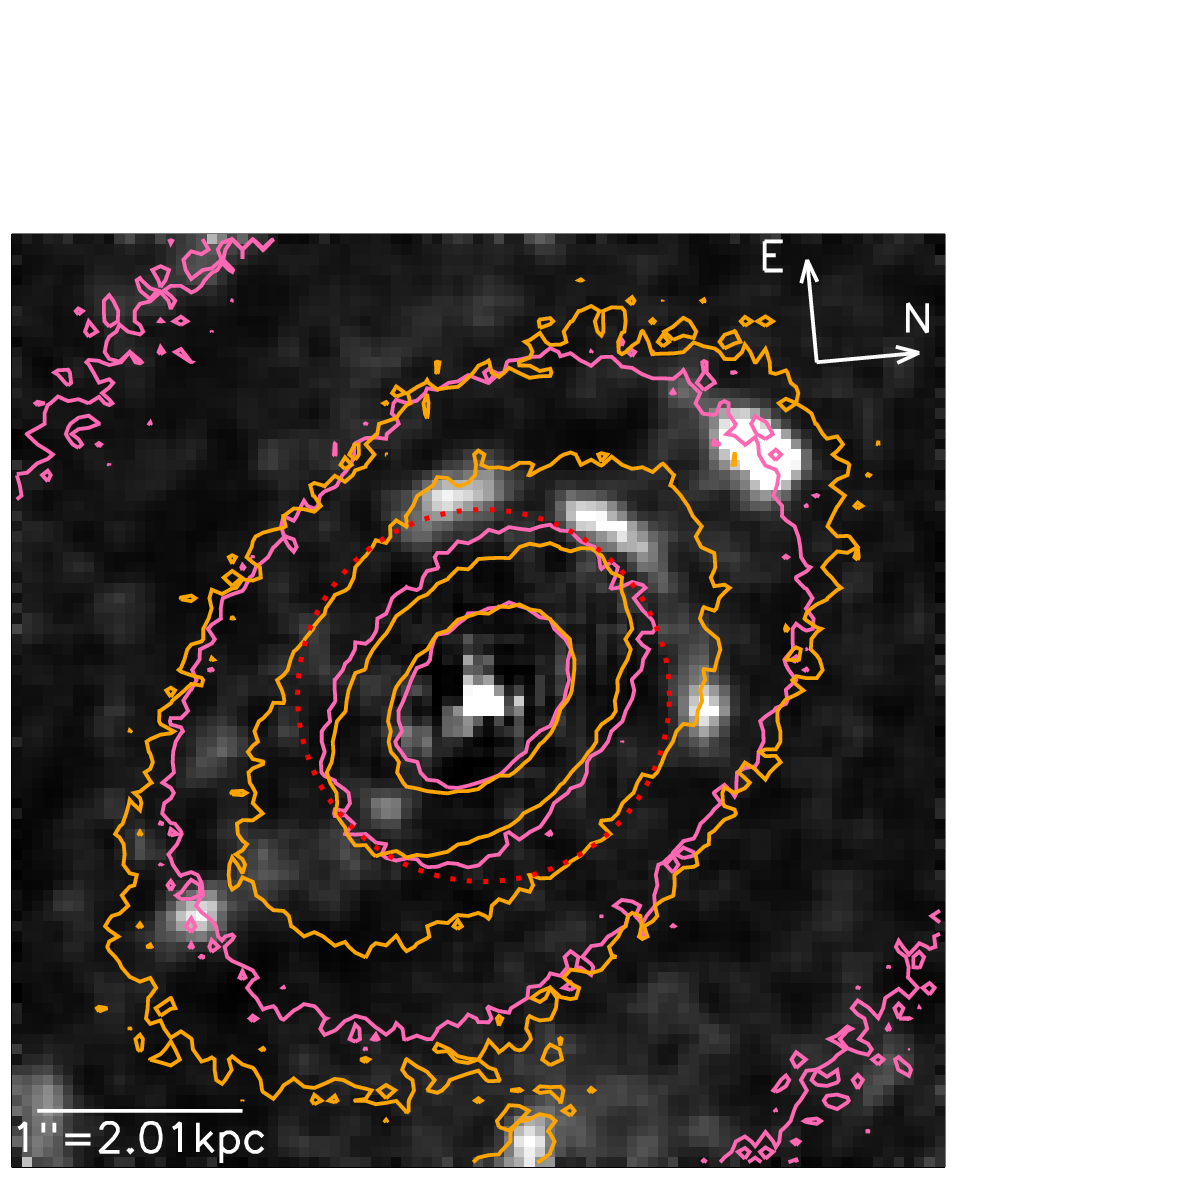
\includegraphics[width=.9\linewidth]{fig/paper_lensmass_brightness_compare.ps}
  \caption{Comparison of mass and light.}
  \label{fig:lenscompareboth}
\end{subfigure}
\caption{Comparison of the observed F814W/I-band surface brightness distribution (Panel (a) and orange contours) and predicted mass distribution from lensing constraints (Panel (b) and pink contours). To allow for a qualitative comparison of the contours in Panel (c), the light distribution was turned into a mass distribution by multiplication with the total mass-to-light ratio inside the Einstein radius $\Upsilon_\text{I,tot}^\text{ein}$ in Table \ref{tab:einsteinML}. The Einstein radius is overplotted as red dotted circle. The uncertainties in the mass model in the second column of Table \ref{tab:bestfitlensmodel} were translated into random Monte Carlo noise in the mass contours. The smooth black contours correspond to the best fit model in the first column of Table \ref{tab:bestfitlensmodel}. The background in Panel (c) shows again the surface brightness subtracted center of the galaxy to make the lensing images visible. [TO DO: use $\Upsilon_\text{I,tot}^\text{ein}$ on colorbar]}
\label{fig:lenslightcompareALL}
\end{figure*}
